  \documentclass[xetex,mathserif,serif]{beamer}

\usepackage{xunicode}
\usepackage{xltxtra}
\usepackage{color}
\usepackage{url}
\usepackage{listings}
\usepackage{fontspec}
\usepackage{geometry}
\usepackage{lastpage}
\usepackage{fancyhdr}
\usepackage{amsmath}
\usepackage{amsthm}
\usepackage{amssymb}
\usepackage{blkarray}
\usepackage{multicol}
\usepackage{relsize}

\definecolor{solarized@base03}{HTML}{002B36}
\definecolor{solarized@base02}{HTML}{073642}
\definecolor{solarized@base01}{HTML}{586e75}
\definecolor{solarized@base00}{HTML}{657b83}
\definecolor{solarized@base0}{HTML}{839496}
\definecolor{solarized@base1}{HTML}{93a1a1}
\definecolor{solarized@base2}{HTML}{EEE8D5}
\definecolor{solarized@base3}{HTML}{FDF6E3}
\definecolor{solarized@yellow}{HTML}{B58900}
\definecolor{solarized@orange}{HTML}{CB4B16}
\definecolor{solarized@red}{HTML}{DC322F}
\definecolor{solarized@magenta}{HTML}{D33682}
\definecolor{solarized@violet}{HTML}{6C71C4}
\definecolor{solarized@blue}{HTML}{268BD2}
\definecolor{solarized@cyan}{HTML}{2AA198}
\definecolor{solarized@green}{HTML}{859900}
\definecolor{yaleblue}{HTML}{0E4C92}

\setbeamertemplate{navigation symbols}{}
% \setbeamerfont{title}{family=\old}
% \setbeamerfont{author}{family=\tfont}%
% \setbeamerfont{frametitle}{family=\oldA}
% \setbeamerfont{date}{family=\dfont}

\setbeamertemplate{itemize items}{--}
\setbeamercolor*{item}{fg=black}

\defaultfontfeatures{Mapping=tex-text}
\hypersetup{pdfstartview={FitH}}

\newcommand{\old}[1]{\fontspec[Alternate=1,Ligatures={Common}]{Hoefler Text}\fontsize{18pt}{30pt}\selectfont #1}%
\newcommand{\oldA}[1]{\fontspec[Alternate=1,Ligatures={Common, Rare}]{Hoefler Text}\fontsize{12pt}{15pt}\selectfont #1}%
\newcommand{\oldB}[1]{\fontspec[Ligatures={Common}]{Didot}\fontsize{12pt}{15pt}\color{solarized@base02}\selectfont #1}%
\newcommand{\tfont}[1]{\fontspec[Alternate=1,Ligatures={Common}]{Hoefler Text}\fontsize{12pt}{20pt}\selectfont #1}%
\newcommand{\dfont}[1]{\fontspec[Ligatures={Common}]{Didot}\fontsize{12pt}{12pt}\selectfont #1}%

\newcommand{\minimize}{\mathop{\mathrm{minimize}}}
\newcommand{\argmin}{\mathop{\mathrm{arg\,min}}}
\newcommand{\argmax}{\mathop{\mathrm{arg\,max}}}
\newcommand{\st}{\mathop{\mathrm{subject\,\,to}}}

\newcommand\independent{\protect\mathpalette{\protect\independenT}{\perp}}
\def\independenT#1#2{\mathrel{\rlap{$#1#2$}\mkern2mu{#1#2}}}

\setlength{\parindent}{0pt}
\setlength{\parskip}{12pt}

\setromanfont [Ligatures={Common}, Numbers={OldStyle}, Variant=01,
 BoldFont={LinLibertine_RB.otf},
 ItalicFont={LinLibertine_RI.otf},
 BoldItalicFont={LinLibertine_RBI.otf}
 ]{LinLibertine_R.otf}



\begin{document}

%%%%%%%%%%%%%%%%%%%%%%%%%%%%%%%%%%%%%%%%%%%%%%%%%%%
\begin{frame}[fragile] \frametitle{}

\vfill

{\fontsize{0.7cm}{0cm}\selectfont Lecture 11 \\\vspace{0.2cm}
Logistic Regression}\\\vspace{0.5cm}
14 October 2015

\vspace{2cm}

\begin{minipage}{0.6\textwidth}
Taylor B. Arnold \\
Yale Statistics \\
STAT 312/612
\end{minipage}
\hfill
\begin{minipage}{0.3\textwidth}\raggedleft

\includegraphics[scale=0.3]{../yale-logo.png}
\end{minipage}%

\end{frame}

%%%%%%%%%%%%%%%%%%%%%%%%%%%%%%%%%%%%%%%%%%%%%%%%%%%
\begin{frame}[fragile] \frametitle{}

{\color{yaleblue}\fontsize{16pt}{20pt}\selectfont Notes}

\begin{itemize}
\item Problem Set \#4 - Due in two weeks
\item No class next Monday
\end{itemize}

\end{frame}

%%%%%%%%%%%%%%%%%%%%%%%%%%%%%%%%%%%%%%%%%%%%%%%%%%%
\begin{frame}[fragile] \frametitle{}

{\color{yaleblue}\fontsize{16pt}{20pt}\selectfont Goals for today}

\begin{itemize}
\item Logistic regression introduction
\item Solving via least squares
\item Running GLMs in R
\end{itemize}

\end{frame}

%%%%%%%%%%%%%%%%%%%%%%%%%%%%%%%%%%%%%%%%%%%%%%%%%%%
\begin{frame}[fragile] \frametitle{}

\begin{flushright}
{\color{yaleblue}\sc\fontsize{1cm}{0cm}\selectfont Logistic regression introduction}
\end{flushright}

\end{frame}

%%%%%%%%%%%%%%%%%%%%%%%%%%%%%%%%%%%%%%%%%%%%%%%%%%%
\begin{frame}[fragile] \frametitle{}

Consider the case where $y_i \in \{0,1\}$ for all values of $i$.
If we write:
\begin{align*}
y &= X \beta + \epsilon
\end{align*}
Why does it not make sense for $\epsilon$ to be independent of X?

\end{frame}

%%%%%%%%%%%%%%%%%%%%%%%%%%%%%%%%%%%%%%%%%%%%%%%%%%%
\begin{frame}[fragile] \frametitle{}

A natural extension of the classical linear regression to handle
this case is, then:
\begin{align*}
\mathbb{E} (y | X) &= g^{-1} \left( X \beta \right)
\end{align*}
For some fixed and known function $g$, called the \textit{link function}.

\pause If $g$ is the identity how does this relate the linear case?

\end{frame}

%%%%%%%%%%%%%%%%%%%%%%%%%%%%%%%%%%%%%%%%%%%%%%%%%%%
\begin{frame}[fragile] \frametitle{}

If $y_i$ has a Bernoilli distribution, notice that this has only one
unknown parameter $p_i = \mathbb{P} (y = 1)$. We can write the likelihood
function as (just plug in the two possible values of $y$ to see that this
works):
\begin{align*}
L(y_i | p_i) &= p_i^{y_i} \cdot (1 - p_i)^{1 - y_i}
\end{align*}
\pause Manipulating this a bit, we can write the likelihood as an exponential
family:
\begin{align*}
L(y_i | p_i) &= (1 - p_i) \cdot \left( \frac{p_i}{1 - p_i} \right)^{y_i}\\
&= (1 - p_i) \cdot \text{exp} \left( y_i \cdot {\color{solarized@red} \text{log} \left( \frac{p_i}{1 - p_i} \right)} \right)
\end{align*}

\end{frame}

%%%%%%%%%%%%%%%%%%%%%%%%%%%%%%%%%%%%%%%%%%%%%%%%%%%
\begin{frame}[fragile] \frametitle{}

I won't derive the entire theory of exponential families today, but this form
suggests that the `canonical' parameter in the Bernoilli distribution is:
\begin{align*}
\eta_i &= \text{log} \left( \frac{p_i}{1 - p_i} \right) \\
&= \text{logit} (p_i)
\end{align*}
\pause Therefore, a natural choice is to say that $\eta_i$ is a linear function
of $x_i$:
\begin{align*}
\eta_i &= x_i^t \beta
\end{align*}
In other words, $g$ is equal to the logit function.

\end{frame}

%%%%%%%%%%%%%%%%%%%%%%%%%%%%%%%%%%%%%%%%%%%%%%%%%%%
\begin{frame}[fragile] \frametitle{}

Now, consider determining the mean of $y_i$ given a regression
vector $\beta$:
\begin{align*}
\text{log} \left( \frac{p_i}{1 - p_i} \right) &= x_i^t \beta \\
\frac{p_i}{1 - p_i} &= e^{x_i^t \beta} \\
p_i &= (1 - p_i) \cdot e^{x_i^t \beta} \\
\left( 1 + e^{x_i^t \beta} \right) p_i &= e^{x_i^t \beta} \\
p_i &= \frac{e^{x_i^t \beta}}{1 + e^{x_i^t \beta}} \\
&= \frac{1}{1 + e^{-x_i^t \beta}}
\end{align*}

\end{frame}

%%%%%%%%%%%%%%%%%%%%%%%%%%%%%%%%%%%%%%%%%%%%%%%%%%%
\begin{frame}[fragile] \frametitle{}

What does the relationship between $x^t \beta$ and $p_i$ look like?

\begin{center}
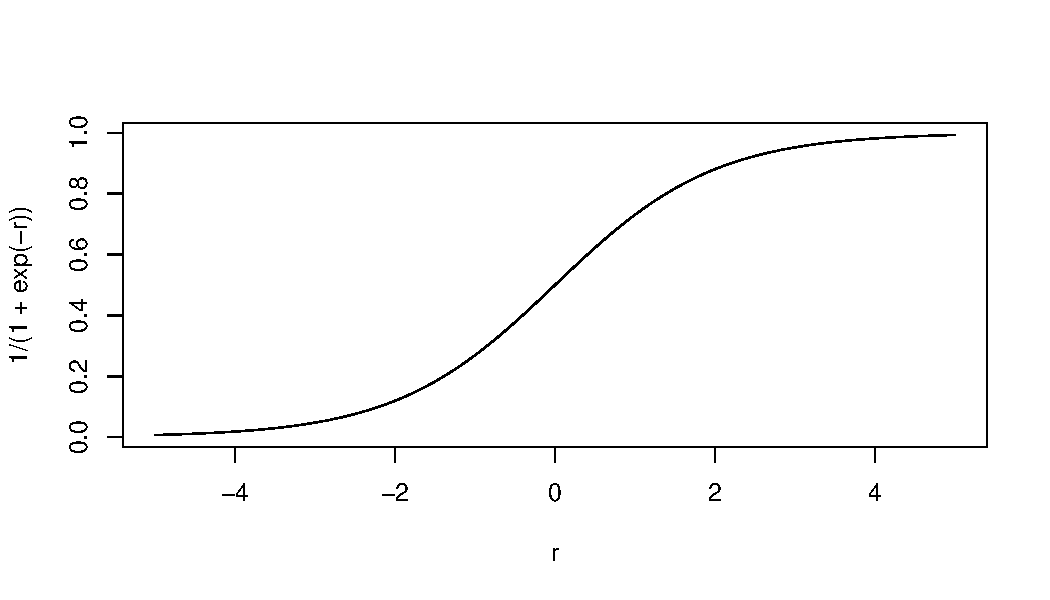
\includegraphics[width=\textwidth]{img/fig01.pdf}
\end{center}

\end{frame}

%%%%%%%%%%%%%%%%%%%%%%%%%%%%%%%%%%%%%%%%%%%%%%%%%%%
\begin{frame}[fragile] \frametitle{}

Note: we could use other link functions $g$, the logit is simply
a popular choice given the theoretical connections to exponential
families.

\end{frame}

%%%%%%%%%%%%%%%%%%%%%%%%%%%%%%%%%%%%%%%%%%%%%%%%%%%
\begin{frame}[fragile] \frametitle{}

\begin{flushright}
{\color{yaleblue}\sc\fontsize{1cm}{0cm}\selectfont Parameter estimation}
\end{flushright}

\end{frame}

%%%%%%%%%%%%%%%%%%%%%%%%%%%%%%%%%%%%%%%%%%%%%%%%%%%
\begin{frame}[fragile] \frametitle{}

The parameters in logistic regression are generally fit using maximum
likelihood estimation. The likelihood for the entire model, building
on what we saw before, is given by:
\begin{align*}
L(y | X) &= \prod_i p_i^{y_i} \cdot (1 - p_i)^{1 - y_i}
\end{align*}
\pause And therefore the log-likelihood is:
\begin{align*}
l(y | X) &= \sum_i \left\{ y_i \cdot \log(p_i) + (1 - y_i) \cdot \log(1 - p_i) \right\} \\
&= \sum_i \left\{ y_i \beta^t x_i - \log\left( 1 + e^{\beta^t x_i} \right) \right\}
\end{align*}

\end{frame}

%%%%%%%%%%%%%%%%%%%%%%%%%%%%%%%%%%%%%%%%%%%%%%%%%%%
\begin{frame}[fragile] \frametitle{}

To find critical points of this,
we set the first derivatives of the log-likelihood with respect to $\beta$
to zero:
\begin{align*}
\frac{\partial}{\partial \beta} l(\beta) &= \sum_i x_i \cdot (y_i - p_i(\beta)) = 0
\end{align*}


\end{frame}


\end{document}











